\documentclass[11pt,a4paper]{article}

% ── packages ──────────────────────────────────────────────────────────────────
\usepackage[T1]{fontenc}
\usepackage[utf8]{inputenc}
\usepackage{lmodern}
\usepackage[margin=2.5cm]{geometry}
\usepackage{amsmath,amssymb,mathtools,bm}
\usepackage{listings}
\usepackage{xcolor}
\usepackage{tikz}
\usetikzlibrary{
  arrows.meta,
  positioning,
  fit,
  shapes.geometric,
  shapes.multipart,
  backgrounds,
  calc,
  decorations.pathreplacing
}
\usepackage{hyperref}
\usepackage{booktabs}
\usepackage{caption}
\usepackage{tcolorbox}
\tcbuselibrary{skins,breakable}

% ── colours ───────────────────────────────────────────────────────────────────
\definecolor{codeblue}{RGB}{0,102,204}
\definecolor{codegray}{RGB}{100,100,100}
\definecolor{codegreen}{RGB}{0,128,64}
\definecolor{codepurple}{RGB}{128,0,128}
\definecolor{backcolour}{RGB}{250,250,250}
\definecolor{nodeblue}{RGB}{173,216,230}
\definecolor{nodeorange}{RGB}{255,200,130}
\definecolor{nodegreen}{RGB}{180,230,180}
\definecolor{adjcolor}{RGB}{220,80,40}
\definecolor{tangcolor}{RGB}{40,100,200}

% ── listings style ────────────────────────────────────────────────────────────
\lstdefinestyle{cpp}{
  backgroundcolor=\color{backcolour},
  commentstyle=\color{codegreen}\itshape,
  keywordstyle=\color{codeblue}\bfseries,
  numberstyle=\tiny\color{codegray},
  stringstyle=\color{codepurple},
  basicstyle=\ttfamily\small,
  breaklines=true,
  captionpos=b,
  keepspaces=true,
  numbers=left,
  numbersep=6pt,
  tabsize=2,
  language=C++,
  morekeywords={constexpr,consteval,concept,requires,auto,typename,template,
                decltype,using,size_t,inline,nodiscard,
                class,struct,namespace,public,private,friend,const,void,bool},
  escapeinside={(*}{*)},
  % Replace Unicode em-dash with LaTeX equivalent inside listings
  literate={---}{{---}}3,
}
\lstset{style=cpp}

% ── tcolorbox helpers ─────────────────────────────────────────────────────────
% NOTE: all callers that pass a title containing $math$ or commas MUST use
%       double braces:  \begin{tcolorbox}[defbox={{title with $math$}}]
\tcbset{
  defbox/.style={
    enhanced,colback=blue!5!white,colframe=blue!50!black,
    fonttitle=\bfseries,title={#1},breakable
  },
  rulebox/.style={
    enhanced,colback=orange!8!white,colframe=orange!70!black,
    fonttitle=\bfseries,title={#1},breakable
  },
  exbox/.style={
    enhanced,colback=green!5!white,colframe=green!50!black,
    fonttitle=\bfseries,title={#1},breakable
  }
}

% ── macros ────────────────────────────────────────────────────────────────────
\newcommand{\code}[1]{\texttt{#1}}
\newcommand{\pf}[2]{\dfrac{\partial #1}{\partial #2}}

\title{%
  \textbf{Forward and Reverse Mode AD}\\[4pt]
  \large Jacobian Computation in \texttt{Expression\_Differentiator}\\[2pt]
  \normalsize A method-by-method walkthrough with worked examples
}
\author{Expression\_Differentiator --- internal documentation}
\date{}

% ══════════════════════════════════════════════════════════════════════════════
\begin{document}
\maketitle
\tableofcontents
\bigskip

% ══════════════════════════════════════════════════════════════════════════════
\section{Introduction}

This document explains how the library computes Jacobians (first-order
derivatives) using \emph{forward-mode} and \emph{reverse-mode} automatic
differentiation (AD).  Every concept is grounded in the actual C++ types, with
line references to the source.

\medskip
\noindent\textbf{Running example.}  Throughout, we use the scalar function of
two variables
\[
  f(x,\,y) \;=\; x\,y \;+\; \sin(x),
  \qquad (x,y) = \left(\tfrac{\pi}{2},\;3\right).
\]
Its Jacobian (gradient row-vector) is
\[
  \nabla f = \begin{pmatrix} \pf{f}{x} & \pf{f}{y} \end{pmatrix}
           = \begin{pmatrix} y + \cos x & x \end{pmatrix}
  \;\Big|_{x=\pi/2,\,y=3}
  = \begin{pmatrix} 3 + 0 & \tfrac{\pi}{2} \end{pmatrix}
  = \begin{pmatrix} 3 & \tfrac{\pi}{2} \end{pmatrix}.
\]

% ══════════════════════════════════════════════════════════════════════════════
\section{Expression Tree Representation}

\subsection{Node types}

Every expression is an immutable tree of nodes.  There is no virtual dispatch;
nodes communicate through C++20 concepts.

\begin{table}[h]
\centering\small
\renewcommand{\arraystretch}{1.3}
\begin{tabular}{lll}
\toprule
\textbf{Node type} & \textbf{Template signature} & \textbf{Role} \\
\midrule
\code{Constant<T>}              & \code{Numeric T}                     & Fixed numeric literal \\
\code{Variable<T,symbol>}       & \code{Numeric T},\;\code{char symbol} & Named mutable scalar \\
\code{RuntimeVariable<T>}       & \code{Numeric T}                     & Index-addressed variable \\
\code{Expression<Op,LHS,RHS>}   & binary op, two child nodes           & Binary operation node \\
\code{MonoExpression<Op,Expr>}  & unary op, one child node             & Unary operation node \\
\code{EvalResult<T>}            & \code{Numeric T}                     & Thin value wrapper \\
\bottomrule
\end{tabular}
\caption{First-class expression node types (\texttt{expressions.hpp}, \texttt{values.hpp}).}
\end{table}

The concept \code{ExpressionConcept} is satisfied by all rows above via the
\code{is\_expression\_type} tag trait (\texttt{expressions.hpp:38--67}).

\subsection{Tree for the running example}

\begin{center}
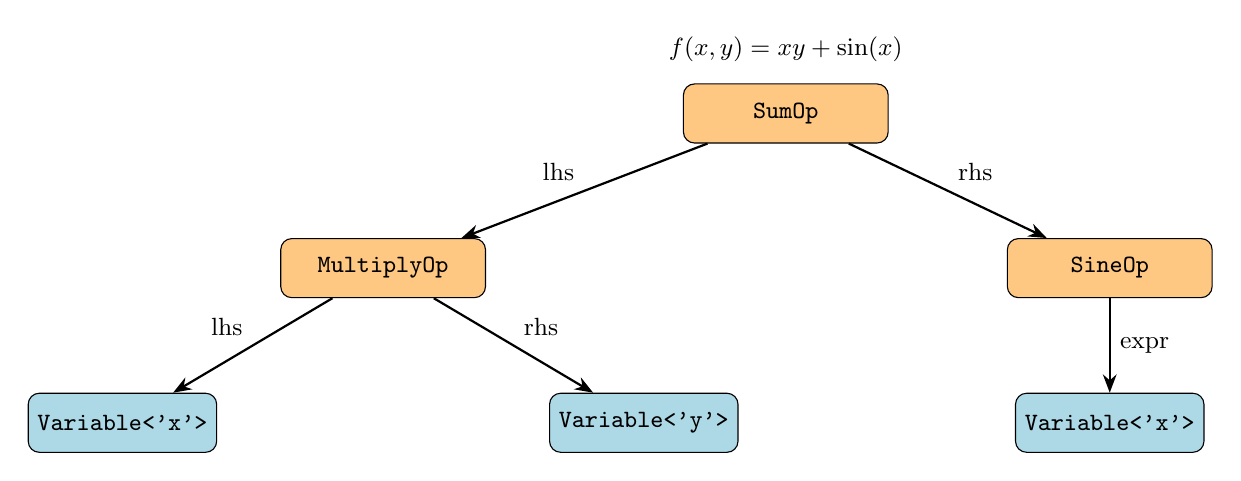
\begin{tikzpicture}[
  node distance=1.4cm and 1.8cm,
  op/.style={draw,rounded corners,fill=nodeorange,minimum width=2.6cm,
             minimum height=0.75cm,font=\ttfamily\small,align=center},
  leaf/.style={draw,rounded corners,fill=nodeblue,minimum width=2.2cm,
               minimum height=0.75cm,font=\ttfamily\small,align=center},
  edge/.style={-{Stealth},thick},
]
\node[op]   (root) {\code{SumOp}};
\node[op,   below left=1.2cm and 2.5cm of root]  (mul)  {\code{MultiplyOp}};
\node[op,   below right=1.2cm and 1.5cm of root] (sine) {\code{SineOp}};
\node[leaf, below left=1.2cm and 0.8cm of mul]   (x1)   {\code{Variable<'x'>}};
\node[leaf, below right=1.2cm and 0.8cm of mul]  (y)    {\code{Variable<'y'>}};
\node[leaf, below=1.2cm of sine]                 (x2)   {\code{Variable<'x'>}};

\draw[edge] (root) -- (mul)  node[midway,above left, font=\small]{lhs};
\draw[edge] (root) -- (sine) node[midway,above right,font=\small]{rhs};
\draw[edge] (mul)  -- (x1)  node[midway,above left, font=\small]{lhs};
\draw[edge] (mul)  -- (y)   node[midway,above right,font=\small]{rhs};
\draw[edge] (sine) -- (x2)  node[midway,right,      font=\small]{expr};

\node[above=0.15cm of root,font=\small\itshape]{$f(x,y) = xy + \sin(x)$};
\end{tikzpicture}
\end{center}

\noindent The symbol \code{'x'} appears in two leaves.  Both have type
\code{Variable<T,'x'>} and are updated in sync by \code{update()}.

\subsection{Universal methods on every node}

Every node unconditionally provides these five methods:

\begin{tcolorbox}[defbox={Method overview}]
\begin{lstlisting}
// 1. Evaluate: returns scalar at current variable state.
auto eval() const -> value_type;

// 2. Walk tree and write new values into every Variable.
void update(const auto& symbols, const auto& updates);

// 3. Walk tree and read current Variable values into an array.
void collect(const auto& symbols, auto& out) const;

// 4. Stateless evaluation from an explicit seed array (no mutation).
template<typename Syms, size_t N>
auto eval_seeded(const array<value_type,N>& vals) const -> value_type;

// 5. Reverse-mode adjoint propagation.
void backward(const auto& syms, value_type adj, auto& grads) const;
\end{lstlisting}
\end{tcolorbox}

% ──────────────────────────────────────────────────────────────────────────────
\subsection{\texttt{eval()}}
\label{sec:eval}

\textbf{Purpose.} Recursively evaluate the expression tree, returning the
scalar primal value.

\medskip\noindent\textbf{Per-node behaviour:}
\begin{itemize}
  \item \code{Constant}: returns stored literal (\texttt{values.hpp:176}).
  \item \code{Variable<T,C>}: returns internal \code{value} (\texttt{values.hpp:218}).
  \item \code{RuntimeVariable}: returns \code{value\_} (\texttt{values.hpp:311}).
  \item \code{Expression<Op,L,R>}: calls \code{Op::eval(lhs, rhs)} via
    \code{std::apply}; delegates to the C++ operator
    (e.g.\ \code{std::plus<T>\{\}}) (\texttt{expressions.hpp:162}).
  \item \code{MonoExpression<Op,E>}: calls \code{Op::eval(expression)}
    (\texttt{expressions.hpp:107}).
\end{itemize}

% NOTE: double braces protect the comma inside \pi/2,\;y=3 from pgfkeys
\begin{tcolorbox}[exbox={{Example: $f(\pi/2,\,3)$}}]
\[
  \texttt{root.eval()}
  \;=\; \underbrace{x \cdot y}_{\texttt{mul.eval()}}
  \;+\; \underbrace{\sin(x)}_{\texttt{sine.eval()}}
  \;=\; \tfrac{\pi}{2}\cdot3 \;+\; 1
  \;=\; \tfrac{3\pi}{2}+1 \;\approx\; 5.712
\]
\end{tcolorbox}

% ──────────────────────────────────────────────────────────────────────────────
\subsection{\texttt{update(symbols, updates)}}
\label{sec:update}

\textbf{Purpose.} Walk the tree and write new values into every \code{Variable}
node belonging to the symbol list \code{symbols}.

\medskip
\noindent\code{symbols} is a Boost.MP11 compile-time type-list
\code{mp\_list<integral\_constant<char,C>,...>}, one entry per unique variable.
\code{updates} is an array of \code{value\_type} aligned with that list.

\medskip\noindent\textbf{Per-node behaviour:}
\begin{itemize}
  \item \code{Constant}: no-op (\texttt{values.hpp:184}).
  \item \code{Variable<T,symbol>}: resolves
    $\texttt{constexpr idx} = \texttt{find\_index\_of\_char<symbol,Syms>()}$,
    then \code{*this = updates[idx]} (\texttt{values.hpp:265--270}).
  \item \code{RuntimeVariable}: \code{value\_ = T(updates[index\_])}
    (\texttt{values.hpp:317--319}).
  \item \code{Expression}: recurses into both children
    (\texttt{expressions.hpp:182--185}).
  \item \code{MonoExpression}: recurses into its child
    (\texttt{expressions.hpp:116--118}).
\end{itemize}

\begin{tcolorbox}[rulebox={Key invariant}]
After \code{expr.update(symbols\{\}, seeds)}, every \code{Variable} in the
entire tree has been refreshed.  Calling \code{expr.eval()} afterward reflects
the new values.  This is the mechanism by which forward-mode seeds
\code{Dual} numbers into the tree before each directional-derivative pass.
\end{tcolorbox}

% ──────────────────────────────────────────────────────────────────────────────
\subsection{\texttt{collect(symbols, out)}}
\label{sec:collect}

\textbf{Purpose.} The inverse of \code{update}: snapshot current variable
values \emph{from} the tree into \code{out}.

Used by the no-argument \code{hessian()} overloads to capture the evaluation
point before reseeding.

\begin{itemize}
  \item \code{Constant}: no-op.
  \item \code{Variable<T,symbol>}: \code{out[idx] = value}
    (\texttt{values.hpp:272--278}).
  \item \code{RuntimeVariable}: no-op (\texttt{values.hpp:320}).
  \item \code{Expression}/\code{MonoExpression}: recurses.
\end{itemize}

% ──────────────────────────────────────────────────────────────────────────────
\subsection{\texttt{eval\_seeded<Syms>(vals)}}
\label{sec:evalseeded}

\textbf{Purpose.} A \emph{stateless} evaluation that bypasses internal
\code{Variable} fields entirely.  Every \code{Variable} node reads its value
from the caller-supplied array \code{vals} instead.

\medskip\noindent\textbf{Per-node behaviour:}
\begin{itemize}
  \item \code{Constant}: returns literal, ignores \code{vals}
    (\texttt{values.hpp:189}).
  \item \code{Variable<T,symbol>}: \code{return vals[find\_index\_of\_char<symbol,Syms>()]}
    (\texttt{values.hpp:232--235}).
  \item \code{RuntimeVariable}: returns \code{value\_}, ignores \code{vals}
    (\texttt{values.hpp:327}).
  \item \code{Expression<Op,L,R>}: recursively calls \code{eval\_seeded} on
    both children, wraps each result in \code{EvalResult}, calls
    \code{Op::eval} (\texttt{expressions.hpp:172--180}).
  \item \code{MonoExpression<Op,E>}: same pattern with one child
    (\texttt{expressions.hpp:109--114}).
\end{itemize}

\begin{tcolorbox}[rulebox={Why EvalResult?}]
\code{Op::eval} requires its arguments to satisfy \code{ExpressionConcept}.
A bare scalar \code{T} does not.  \code{EvalResult<T>} is a zero-overhead
wrapper that does:
\begin{lstlisting}
template <Numeric T> struct EvalResult {  // expressions.hpp:59-64
  T value;
  constexpr T eval() const { return value; }
  constexpr operator T() const { return value; }
};
\end{lstlisting}
It satisfies \code{ExpressionConcept} yet carries only a scalar, allowing
\code{eval\_seeded} to reuse the exact same \code{Op::eval} path as
\code{eval()} with no code duplication.  The compiler eliminates it entirely.
\end{tcolorbox}

\noindent\code{eval\_seeded} is the workhorse of the \emph{forward-mode
Hessian}, where the expression is \code{const} and must be evaluated at many
different \code{Dual<Dual<T>>} seed arrays without mutating it.

% ──────────────────────────────────────────────────────────────────────────────
\subsection{\texttt{backward(syms, adj, grads)}}
\label{sec:backward}

\textbf{Purpose.} Reverse-mode adjoint propagation.  Given that this node's
output is weighted by the upstream adjoint \code{adj} ($=\partial f/\partial
v$), accumulate each variable's contribution into \code{grads}.

\medskip\noindent\textbf{Parameters:}
\begin{itemize}
  \item \code{syms} --- compile-time symbol list.
  \item \code{adj} --- adjoint flowing \emph{into} this node: how much the
    final output $f$ depends on this node's output.
  \item \code{grads} --- output array; slot $i$ accumulates
    $\partial f/\partial x_i$ via \textbf{additive} \code{+=}.
\end{itemize}

\medskip\noindent\textbf{Per-node behaviour:}

\paragraph{Constant.}
No variable, no contribution.
\begin{lstlisting}
constexpr void backward(const auto&, T, auto&) const {}  // values.hpp:186
\end{lstlisting}

\paragraph{Variable$\langle$T,symbol$\rangle$.}
This is a leaf: $\partial(\text{self})/\partial x_{\text{self}} = 1$,
so accumulate the full adjoint.
\begin{lstlisting}
// values.hpp:286-292
constexpr void backward(const auto& syms, T adj, auto& grads) const {
    constexpr auto idx = find_index_of_char<symbol, Syms>();
    grads[idx] += adj;
}
\end{lstlisting}

\paragraph{RuntimeVariable.}
\code{grads[index\_] += adj} (\texttt{values.hpp:322--324}).

\paragraph{Expression$\langle$Op,L,R$\rangle$.}
Delegates to \code{Op::backward(lhs, rhs, adj, syms, grads)}
(\texttt{expressions.hpp:190--193}).

\paragraph{MonoExpression$\langle$Op,E$\rangle$.}
Delegates to \code{Op::backward(expression, adj, syms, grads)}
(\texttt{expressions.hpp:122--124}).

% ──────────────────────────────────────────────────────────────────────────────
\subsection{Operation-level \texttt{backward} rules}
\label{sec:opbackward}

Each \code{Op} struct's \code{backward} method encodes the chain rule for one
mathematical operation.

\begin{tcolorbox}[defbox={{SumOp: $f = u + v$}}]
$\pf{f}{u} = 1,\;\pf{f}{v} = 1$\;--- both children get the adjoint unchanged.
\begin{lstlisting}
lhs.backward(syms, adj, grads);  // operations.hpp:65
rhs.backward(syms, adj, grads);  // operations.hpp:66
\end{lstlisting}
\end{tcolorbox}

\begin{tcolorbox}[defbox={{MultiplyOp: $f = u \cdot v$}}]
$\pf{f}{u} = v,\;\pf{f}{v} = u$\;--- each child is scaled by the other operand's value.
\begin{lstlisting}
lhs.backward(syms, adj * static_cast<T>(rhs), grads);  // operations.hpp:81
rhs.backward(syms, adj * static_cast<T>(lhs), grads);  // operations.hpp:82
\end{lstlisting}
\end{tcolorbox}

\begin{tcolorbox}[defbox={{DivideOp: $f = u / v$}}]
$\pf{f}{u} = 1/v,\;\pf{f}{v} = -u/v^2$:
\begin{lstlisting}
const T b = static_cast<T>(rhs);            // operations.hpp:108-114
lhs.backward(syms, adj / b, grads);
rhs.backward(syms, -adj * static_cast<T>(lhs) / (b * b), grads);
\end{lstlisting}
\end{tcolorbox}

\begin{tcolorbox}[defbox={{NegateOp: $f = -u$}}]
\begin{lstlisting}
expr.backward(syms, -adj, grads);  // df/du = -1
\end{lstlisting}
\end{tcolorbox}

\begin{tcolorbox}[defbox={{SineOp: $f = \sin(u)$}}]
\begin{lstlisting}
expr.backward(syms, adj * cos(static_cast<T>(expr)), grads); // df/du = cos(u)
\end{lstlisting}
\end{tcolorbox}

\begin{tcolorbox}[defbox={{ExpOp: $f = e^u$}}]
\begin{lstlisting}
expr.backward(syms, adj * exp(static_cast<T>(expr)), grads); // df/du = e^u
\end{lstlisting}
\end{tcolorbox}

\noindent All other transcendentals follow the same pattern.

\begin{table}[h]
\centering\small
\renewcommand{\arraystretch}{1.3}
\begin{tabular}{llll}
\toprule
\textbf{Op} & $f(u)$ & local $\partial f/\partial u$ & multiplier on \code{adj} \\
\midrule
\code{NegateOp}  & $-u$         & $-1$              & $-\texttt{adj}$ \\
\code{SineOp}    & $\sin u$     & $\cos u$          & \code{adj*cos(u)} \\
\code{CosineOp}  & $\cos u$     & $-\sin u$         & \code{-adj*sin(u)} \\
\code{ExpOp}     & $e^u$        & $e^u$             & \code{adj*exp(u)} \\
\code{TanOp}     & $\tan u$     & $\sec^2 u$        & \code{adj/(cos(u)$^2$)} \\
\code{LogOp}     & $\ln u$      & $1/u$             & \code{adj/u} \\
\code{SqrtOp}    & $\sqrt{u}$   & $1/(2\sqrt{u})$   & \code{adj/(2*sqrt(u))} \\
\code{AbsOp}     & $|u|$        & $\text{sign}(u)$  & \code{adj*sign(u)} \\
\code{SinhOp}    & $\sinh u$    & $\cosh u$         & \code{adj*cosh(u)} \\
\code{CoshOp}    & $\cosh u$    & $\sinh u$         & \code{adj*sinh(u)} \\
\code{TanhOp}    & $\tanh u$    & $\text{sech}^2 u$ & \code{adj/(cosh(u)$^2$)} \\
\code{AsinOp}    & $\arcsin u$  & $1/\sqrt{1-u^2}$  & \code{adj/sqrt(1-u*u)} \\
\code{AcosOp}    & $\arccos u$  & $-1/\sqrt{1-u^2}$ & \code{-adj/sqrt(1-u*u)} \\
\code{AtanOp}    & $\arctan u$  & $1/(1+u^2)$       & \code{adj/(1+u*u)} \\
\bottomrule
\end{tabular}
\caption{All unary \texttt{backward} rules (\texttt{operations.hpp}).}
\end{table}

% ══════════════════════════════════════════════════════════════════════════════
\section{Dual Numbers --- the Engine of Forward Mode}
\label{sec:dual}

\subsection{Definition}

A \emph{dual number} is a pair $(v,\,\dot{v})$ where $v$ is the primal value
and $\dot{v}$ is the tangent.  Arithmetic extends ordinary arithmetic by
$\varepsilon^2 = 0$:
\[
  (v,\dot v)+(u,\dot u) = (v+u,\;\dot v+\dot u)
\]
\[
  (v,\dot v)\cdot(u,\dot u) = (vu,\;\dot{v}u+v\dot{u})
  \qquad\text{(product rule)}
\]
\[
  \frac{(v,\dot v)}{(u,\dot u)} = \left(\frac{v}{u},\;\frac{\dot{v}u-v\dot{u}}{u^2}\right)
  \qquad\text{(quotient rule)}
\]

\subsection{Implementation: \texttt{Dual<T>} (\texttt{dual.hpp})}

\begin{lstlisting}
template <typename T> class Dual {
    T val{};    // primal
    T deriv{};  // tangent

    constexpr Dual operator*(const Dual& o) const {    // dual.hpp:26-28
        return Dual{val*o.val,  deriv*o.val + val*o.deriv};  // product rule
    }
};

// Transcendentals apply the chain rule automatically:
friend constexpr Dual sin(const Dual& d) {             // dual.hpp:68-71
    return Dual{sin(d.val),  cos(d.val) * d.deriv};
}
friend constexpr Dual exp(const Dual& d) {             // dual.hpp:77-79
    const T e = exp(d.val);
    return Dual{e,  e * d.deriv};
}
\end{lstlisting}

\code{Dual<T>} satisfies the \code{Numeric} concept (\texttt{dual.hpp:127}),
so \code{Variable<Dual<double>,'x'>} is a perfectly ordinary expression node
whose value happens to carry a tangent.

\subsection{Component access}

\code{Dual<T>::get<I>()} returns \code{val} ($I=0$) or \code{deriv} ($I=1$).
For nested \code{Dual<Dual<T>>} (Hessians):
\code{.get<1>().get<1>()} extracts the second-order derivative.

% ══════════════════════════════════════════════════════════════════════════════
\section{Forward-Mode Jacobian}
\label{sec:fwdmode}

\subsection{Mathematical basis}

For $f:\mathbb{R}^n\to\mathbb{R}$, the $j$-th column $\partial f/\partial x_j$
of the Jacobian is obtained by seeding the $j$-th tangent to 1 and all others
to 0:
\[
  f\!\left((x_1,0),\ldots,(x_j,1),\ldots,(x_n,0)\right)
  = \!\left(f(\mathbf{x}),\;\pf{f}{x_j}\right).
\]
Dual arithmetic propagates this tangent through every operation automatically.
The full Jacobian requires $n$ passes.

\subsection{Code walkthrough: \texttt{detail::forward\_mode\_gradient}}
\label{sec:fwdcode}

\textbf{Location:} \texttt{gradient.hpp:58--91}.

\begin{lstlisting}
template <ExpressionConcept Expr, ...>
auto forward_mode_gradient(Expr& expr, array<TArr, N> values)
    requires is_dual_v<typename Expr::value_type>
{
    using symbols    = extract_symbols_from_expr<Expr>::type;
    constexpr size_t n = mp::mp_size<symbols>::value;

    array<value_type, n>  seeds{};      // (*\color{tangcolor}{Dual seeds pushed into the tree}*)
    array<scalar_type, n> gradients{};  // (*\color{tangcolor}{output}*)

    [&]<size_t... Js>(index_sequence<Js...>) {
        // Step 1: init all to (value_j, 0)
        ((seeds[Js] = value_type{values[Js], scalar_type{}}), ...);

        // Step 2: one pass per variable j
        ([&]() {
            seeds[Js] = value_type{values[Js], scalar_type{1}}; // tangent = 1
            expr.update(symbols{}, seeds);                       // push into tree
            gradients[Js] = expr.eval().template get<1>();       // extract df/dxj
            seeds[Js] = value_type{values[Js], scalar_type{}};  // reset
        }(), ...);
    }(make_index_sequence<n>{});

    expr.update(symbols{}, seeds);   // Step 3: restore zero-tangent state
    return gradients;
}
\end{lstlisting}

\medskip\noindent\textbf{Step by step:}
\begin{enumerate}
  \item \textbf{Initialise seeds.}  All seeds: \code{Dual\{values[i], 0\}}.
  \item \textbf{One pass per $j$ (compile-time loop unroll):}
    \begin{itemize}
      \item Set \code{seeds[j].deriv = 1} (direction $e_j$).
      \item \code{expr.update()} writes all seeds into the tree.
      \item \code{expr.eval()} runs with dual arithmetic throughout.
        The returned \code{Dual} has \code{.get<1>()} $= \partial f/\partial x_j$.
      \item Store into \code{gradients[j]}, reset \code{seeds[j].deriv = 0}.
    \end{itemize}
  \item \textbf{Restore state.}  Final \code{update} leaves the tree
        zero-tangent.
\end{enumerate}

\textbf{Complexity:} $O(n \cdot |E|)$.  Requires $n$ full tree evaluations.

\subsection{Flowchart}

\begin{center}
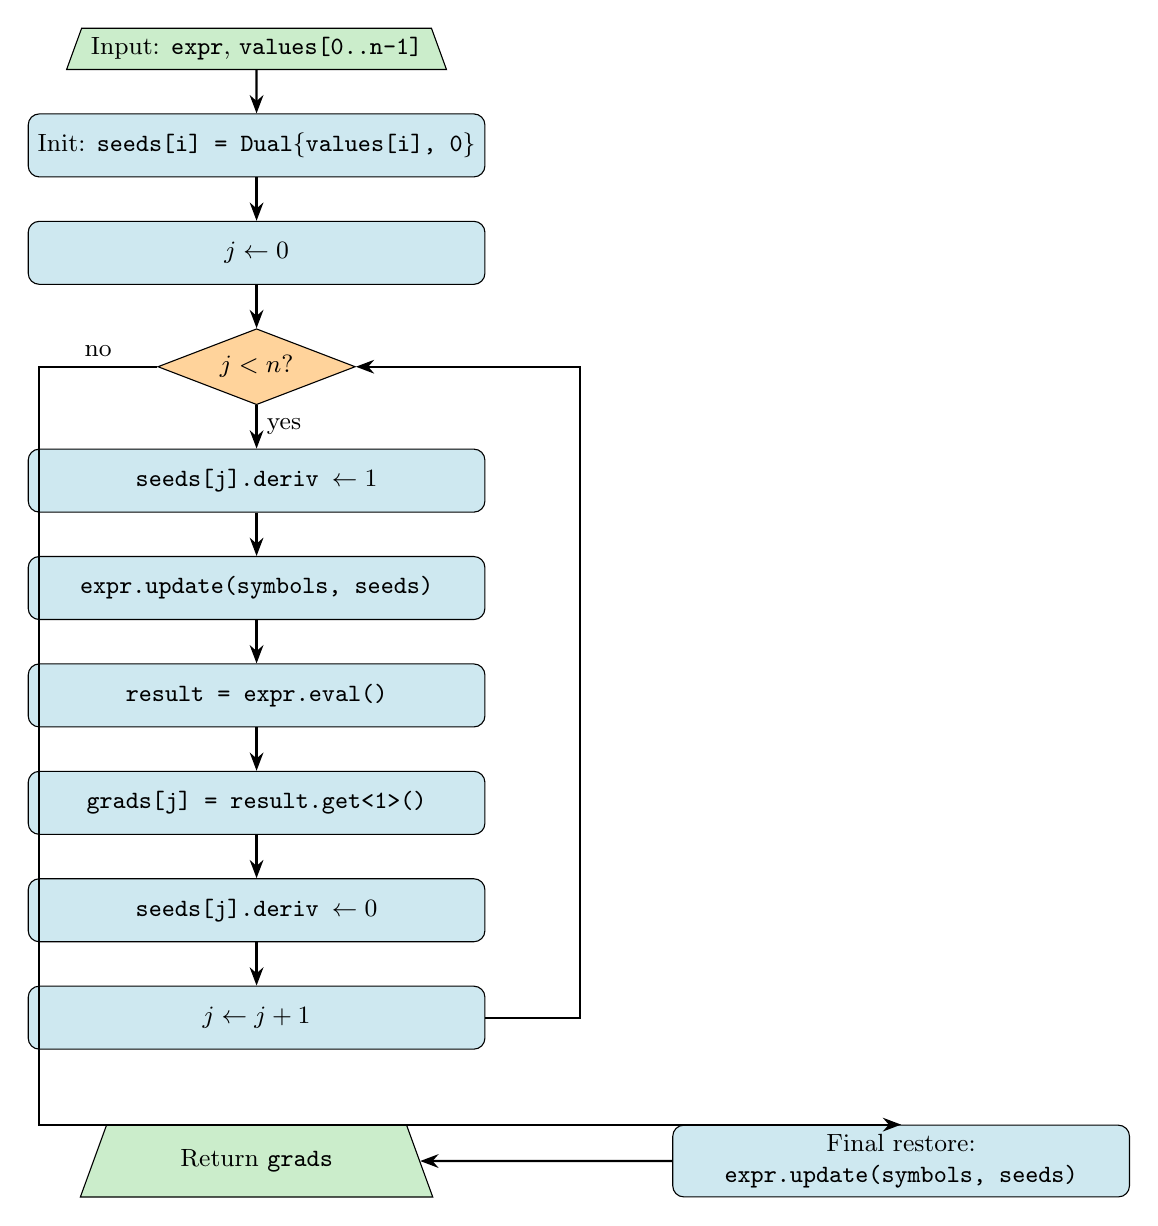
\begin{tikzpicture}[
  block/.style={draw,rounded corners,fill=nodeblue!60,minimum width=5.8cm,
                minimum height=0.8cm,align=center,font=\small},
  decision/.style={draw,diamond,fill=nodeorange!80,aspect=2.6,
                   align=center,font=\small},
  io/.style={draw,trapezium,trapezium left angle=70,trapezium right angle=70,
             fill=nodegreen!70,minimum width=4.5cm,align=center,font=\small},
  arr/.style={-{Stealth},thick},
  node distance=0.55cm,
]
\node[io]       (in)    {Input: \texttt{expr}, \texttt{values[0..n-1]}};
\node[block,below=of in]   (init)  {Init: \texttt{seeds[i] = Dual\{values[i], 0\}}};
\node[block,below=of init] (j0)    {$j \leftarrow 0$};
\node[decision, below=of j0](cond) {$j < n$?};
\node[block,below=of cond] (seed1) {\texttt{seeds[j].deriv $\leftarrow 1$}};
\node[block,below=of seed1](upd)   {\texttt{expr.update(symbols, seeds)}};
\node[block,below=of upd]  (ev)    {\texttt{result = expr.eval()}};
\node[block,below=of ev]   (ext)   {\texttt{grads[j] = result.get<1>()}};
\node[block,below=of ext]  (res)   {\texttt{seeds[j].deriv $\leftarrow 0$}};
\node[block,below=of res]  (inc)   {$j \leftarrow j+1$};
\node[io,   below=of inc, yshift=-0.4cm] (out) {Return \texttt{grads}};
\node[block,right=3.2cm of out] (rst) {Final restore:\\\texttt{expr.update(symbols, seeds)}};

\draw[arr] (in) -- (init);
\draw[arr] (init) -- (j0);
\draw[arr] (j0)   -- (cond);
\draw[arr] (cond) -- node[right,font=\small]{yes} (seed1);
\draw[arr] (seed1)-- (upd);
\draw[arr] (upd)  -- (ev);
\draw[arr] (ev)   -- (ext);
\draw[arr] (ext)  -- (res);
\draw[arr] (res)  -- (inc);
\draw[arr] (inc.east) -- ++(1.2,0) |- (cond.east);
\draw[arr] (cond.west) -- node[above,font=\small]{no} ++(-1.5,0) |- (rst.north);
\draw[arr] (rst) -- (out);
\end{tikzpicture}
\end{center}

\subsection{Worked example}

\subsubsection*{Pass $j=0$: compute $\partial f/\partial x$}

Seeds: $x = (\pi/2,\;1)$,\quad $y = (3,\;0)$

\begin{center}\small
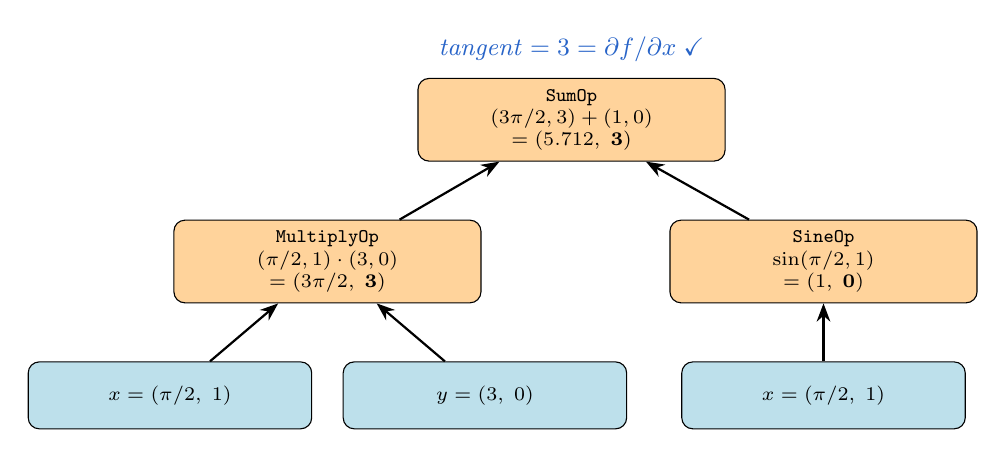
\begin{tikzpicture}[
  op/.style  ={draw,rounded corners,fill=nodeorange!80,minimum width=3.9cm,
               minimum height=1.05cm,font=\ttfamily\scriptsize,align=center},
  leaf/.style={draw,rounded corners,fill=nodeblue!80,minimum width=3.6cm,
               minimum height=0.85cm,font=\ttfamily\scriptsize,align=center},
  arr/.style ={-{Stealth},thick},
]
\node[leaf] (x1) at (-3.8,-3.2) {$x = (\pi/2,\;1)$};
\node[leaf] (y)  at ( 0.2,-3.2) {$y = (3,\;0)$};
\node[leaf] (x2) at ( 4.5,-3.2) {$x = (\pi/2,\;1)$};

\node[op]   (mul)  at (-1.8,-1.5) {\code{MultiplyOp}\\
  $(\pi/2,1)\cdot(3,0)$\\
  $= (3\pi/2,\;\mathbf{3})$};
\node[op]   (sine) at ( 4.5,-1.5) {\code{SineOp}\\
  $\sin(\pi/2,1)$\\
  $= (1,\;\mathbf{0})$};
\node[op]   (root) at ( 1.3, 0.3) {\code{SumOp}\\
  $(3\pi/2,3)+(1,0)$\\
  $= (5.712,\;\mathbf{3})$};

\draw[arr] (x1) -- (mul);
\draw[arr] (y)  -- (mul);
\draw[arr] (x2) -- (sine);
\draw[arr] (mul) -- (root);
\draw[arr] (sine)-- (root);
\node[above=0.08cm of root,font=\small\itshape\color{tangcolor}]
  {tangent $=3 = \partial f/\partial x$\;\checkmark};
\end{tikzpicture}
\end{center}

\noindent\emph{Product rule:}
$\dot{(xy)} = \dot{x}\cdot y + x\cdot\dot{y} = 1\cdot3 + \tfrac{\pi}{2}\cdot0 = 3$.\\
\emph{Chain rule on sine:}
$\dot{\sin x} = \cos(\pi/2)\cdot1 = 0$.\\
Sum: $3+0 = \mathbf{3}$.

\subsubsection*{Pass $j=1$: compute $\partial f/\partial y$}

Seeds: $x = (\pi/2,\;0)$,\quad $y = (3,\;1)$

\begin{center}\small
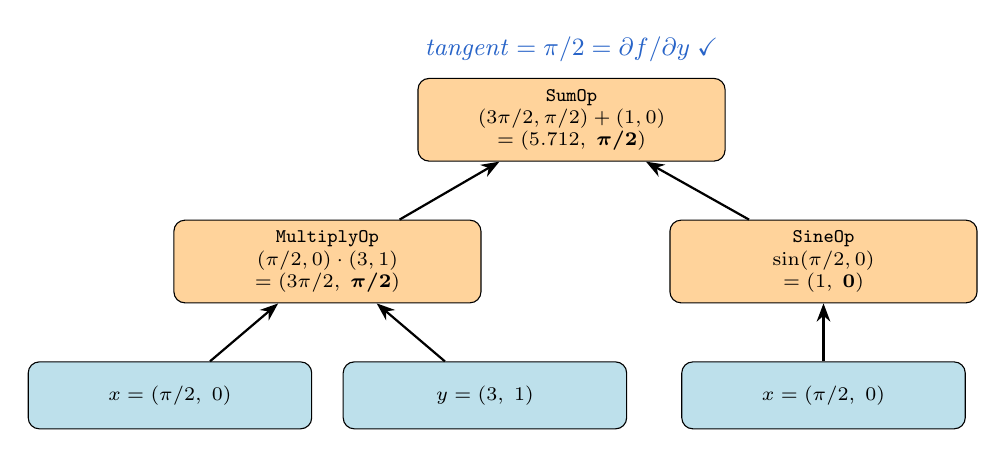
\begin{tikzpicture}[
  op/.style  ={draw,rounded corners,fill=nodeorange!80,minimum width=3.9cm,
               minimum height=1.05cm,font=\ttfamily\scriptsize,align=center},
  leaf/.style={draw,rounded corners,fill=nodeblue!80,minimum width=3.6cm,
               minimum height=0.85cm,font=\ttfamily\scriptsize,align=center},
  arr/.style ={-{Stealth},thick},
]
\node[leaf] (x1) at (-3.8,-3.2) {$x = (\pi/2,\;0)$};
\node[leaf] (y)  at ( 0.2,-3.2) {$y = (3,\;1)$};
\node[leaf] (x2) at ( 4.5,-3.2) {$x = (\pi/2,\;0)$};

\node[op]   (mul)  at (-1.8,-1.5) {\code{MultiplyOp}\\
  $(\pi/2,0)\cdot(3,1)$\\
  $= (3\pi/2,\;\bm{\pi/2})$};
\node[op]   (sine) at ( 4.5,-1.5) {\code{SineOp}\\
  $\sin(\pi/2,0)$\\
  $= (1,\;\mathbf{0})$};
\node[op]   (root) at ( 1.3, 0.3) {\code{SumOp}\\
  $(3\pi/2,\pi/2)+(1,0)$\\
  $= (5.712,\;\bm{\pi/2})$};

\draw[arr] (x1) -- (mul);
\draw[arr] (y)  -- (mul);
\draw[arr] (x2) -- (sine);
\draw[arr] (mul) -- (root);
\draw[arr] (sine)-- (root);
\node[above=0.08cm of root,font=\small\itshape\color{tangcolor}]
  {tangent $=\pi/2 = \partial f/\partial y$\;\checkmark};
\end{tikzpicture}
\end{center}

\noindent\emph{Product rule:}
$\dot{(xy)} = 0\cdot3 + \tfrac{\pi}{2}\cdot1 = \tfrac{\pi}{2}$.

% ══════════════════════════════════════════════════════════════════════════════
\section{Reverse-Mode Jacobian}
\label{sec:revmode}

\subsection{Mathematical basis}

Define the \emph{adjoint} of node $v$ as $\bar{v} = \partial f/\partial v$.
Starting from the output ($\bar{f}=1$), a single backward pass distributes
adjoints to every input node via the chain rule.  For $f = \ell(u,v)$:
\[
  \bar{u} \mathrel{+}= \bar{f}\cdot\pf{\ell}{u},
  \qquad
  \bar{v} \mathrel{+}= \bar{f}\cdot\pf{\ell}{v}.
\]
The $+=$ accumulation automatically handles variables appearing in multiple
places (e.g.\ both $x$ leaves contribute to the same $\bar{x}$).

\subsection{Code walkthrough: \texttt{detail::reverse\_mode\_gradient}}
\label{sec:revcode}

\textbf{Location:} \texttt{gradient.hpp:31--40}.

\begin{lstlisting}
template <ExpressionConcept Expr, typename T = typename Expr::value_type>
    requires (!is_dual_v<T>)
constexpr auto reverse_mode_gradient(const Expr& expr) {
    using Syms = extract_symbols_from_expr<Expr>::type;
    constexpr auto N = mp::mp_size<Syms>::value;
    std::array<T, N> grads{};             // (*\color{adjcolor}{zero-init output}*)
    expr.backward(Syms{}, T{1}, grads);   // (*\color{adjcolor}{seed root adjoint = 1}*)
    return grads;
}
\end{lstlisting}

\medskip\noindent\textbf{Step by step:}
\begin{enumerate}
  \item Allocate \code{grads[0..n-1] = 0}.
  \item Call \code{expr.backward(Syms\{\}, 1, grads)}.  Root adjoint $= 1$
        because $\partial f/\partial f = 1$.
  \item \code{backward} recursively applies the chain rule; at each
        \code{Variable} leaf, \code{grads[idx] += adj} accumulates the result.
  \item Return \code{grads}: element $i$ holds $\partial f/\partial x_i$.
\end{enumerate}

\textbf{Complexity:} $O(|E|)$ --- a single traversal regardless of $n$.
The expression is taken as \code{const Expr\&}; the tree is not mutated.

\subsection{Flowchart}

\begin{center}
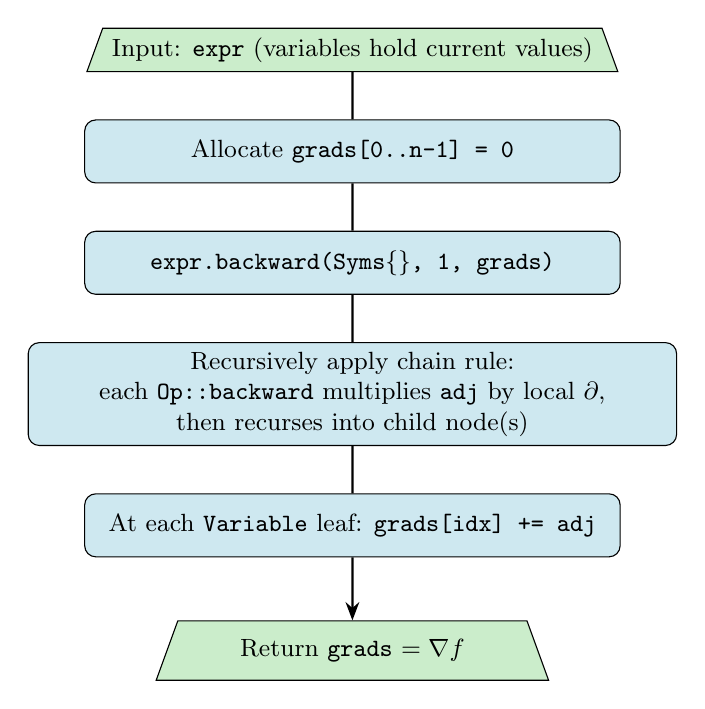
\begin{tikzpicture}[
  block/.style={draw,rounded corners,fill=nodeblue!60,minimum width=6.8cm,
                minimum height=0.8cm,align=center,font=\small},
  io/.style   ={draw,trapezium,trapezium left angle=70,trapezium right angle=70,
                fill=nodegreen!70,minimum width=5cm,align=center,font=\small},
  arr/.style  ={-{Stealth},thick},
  node distance=0.6cm,
]
\node[io]    (in)   {Input: \texttt{expr} (variables hold current values)};
\node[block, below=of in]   (alloc){Allocate \texttt{grads[0..n-1] = 0}};
\node[block, below=of alloc](bk)   {\texttt{expr.backward(Syms\{\}, 1, grads)}};
\node[block, below=of bk, text width=8cm] (rec)
  {Recursively apply chain rule:\\
   each \texttt{Op::backward} multiplies \texttt{adj} by local $\partial$,\\
   then recurses into child node(s)};
\node[block, below=of rec]  (var)  {At each \texttt{Variable} leaf:
                                    \texttt{grads[idx] += adj}};
\node[io,    below=of var, yshift=-0.2cm] (out){Return \texttt{grads} $= \nabla f$};

\draw[arr] (in)--(alloc)--(bk)--(rec)--(var)--(out);
\end{tikzpicture}
\end{center}

\subsection{Worked example}

Variables already hold $x=\pi/2,\;y=3$.  The diagram shows adjoint flow
({\color{adjcolor}dashed orange}) propagating top-down, while structural edges
point bottom-up.

\begin{center}\small
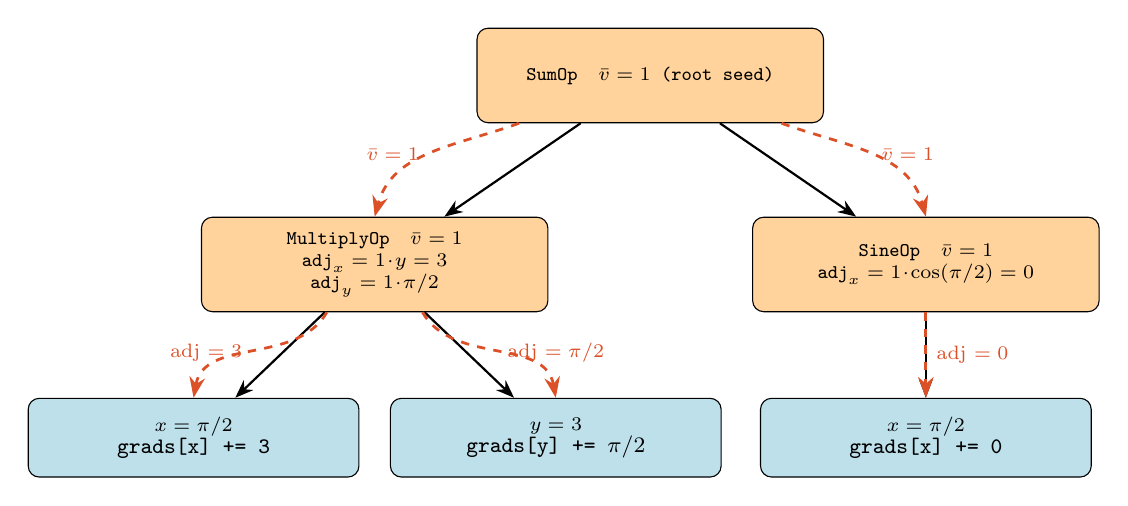
\begin{tikzpicture}[
  op/.style  ={draw,rounded corners,fill=nodeorange!80,minimum width=4.4cm,
               minimum height=1.2cm,font=\ttfamily\scriptsize,align=center},
  leaf/.style={draw,rounded corners,fill=nodeblue!80,minimum width=4.2cm,
               minimum height=1.0cm,font=\ttfamily\scriptsize,align=center},
  fwd/.style ={{Stealth}-,thick,black},
  bwd/.style ={-{Stealth},thick,adjcolor,dashed,line width=1pt},
]
\node[leaf] (x1) at (-4.2,-4.5)
  {$x = \pi/2$\\\footnotesize\texttt{grads[x] += 3}};
\node[leaf] (y)  at ( 0.4,-4.5)
  {$y = 3$\\\footnotesize\texttt{grads[y] += }$\pi/2$};
\node[leaf] (x2) at ( 5.1,-4.5)
  {$x = \pi/2$\\\footnotesize\texttt{grads[x] += 0}};

\node[op]   (mul)  at (-1.9,-2.3)
  {\code{MultiplyOp}\quad $\bar{v}=1$\\
   $\text{adj}_x = 1\!\cdot\!y = 3$\\
   $\text{adj}_y = 1\!\cdot\!\pi/2$};
\node[op]   (sine) at ( 5.1,-2.3)
  {\code{SineOp}\quad $\bar{v}=1$\\
   $\text{adj}_x = 1\!\cdot\!\cos(\pi/2)=0$};
\node[op]   (root) at ( 1.6, 0.1)
  {\code{SumOp}\quad $\bar{v}=1$ (root seed)};

% structural (forward) edges
\draw[fwd] (x1)   -- (mul);
\draw[fwd] (y)    -- (mul);
\draw[fwd] (x2)   -- (sine);
\draw[fwd] (mul)  -- (root);
\draw[fwd] (sine) -- (root);

% adjoint (backward) edges
\draw[bwd] (root.200) to[out=200,in=75]
  node[left, font=\scriptsize\color{adjcolor}]{$\bar{v}=1$} (mul.north);
\draw[bwd] (root.340) to[out=340,in=105]
  node[right,font=\scriptsize\color{adjcolor}]{$\bar{v}=1$} (sine.north);
\draw[bwd] (mul.225)  to[out=240,in=80]
  node[left, font=\scriptsize\color{adjcolor}]{adj $=3$}    (x1.north);
\draw[bwd] (mul.315)  to[out=300,in=100]
  node[right,font=\scriptsize\color{adjcolor}]{adj $=\pi/2$}(y.north);
\draw[bwd] (sine.south) --
  node[right,font=\scriptsize\color{adjcolor}]{adj $=0$}    (x2.north);
\end{tikzpicture}
\end{center}

\noindent\textbf{Accumulation at variable nodes:}
\begin{align*}
  \texttt{grads[x]} &= 3 + 0 = 3 = y+\cos(x)\big|_{\pi/2,3} \checkmark \\
  \texttt{grads[y]} &= \tfrac{\pi}{2} = x \checkmark
\end{align*}

\noindent Both $x$ leaves contribute to the same \code{grads[idx\_x]} slot via
\code{+=} in \code{Variable::backward}.  This is what makes reverse mode exact
when variables appear multiple times in the expression (DAG, not just tree).

% ══════════════════════════════════════════════════════════════════════════════
\section{Comparison}
\label{sec:comparison}

\begin{table}[h]
\centering\small
\renewcommand{\arraystretch}{1.3}
\begin{tabular}{lll}
\toprule
\textbf{Property} & \textbf{Forward mode} & \textbf{Reverse mode} \\
\midrule
Algorithm          & Dual tangent propagation    & Adjoint backpropagation \\
Passes required    & $n$ (one per input)         & $1$ \\
Tree mutation      & Yes (\code{update} per pass) & No (\code{const Expr\&}) \\
Output per pass    & one $\partial f/\partial x_j$ & full $\nabla f$ \\
Time complexity    & $O(n\cdot|E|)$              & $O(|E|)$ \\
Preferred when     & few inputs ($n \ll m$)      & many inputs, scalar $f$ \\
Variable type      & \code{Variable<Dual<T>,'x'>} & \code{Variable<T,'x'>} \\
\bottomrule
\end{tabular}
\caption{Forward vs.\ reverse mode.}
\end{table}

\subsection{Public API (\texttt{gradient.hpp:196--211})}

\begin{lstlisting}
// Reverse mode
auto g1 = gradient<diff::DiffMode::Reverse>(expr);

// Forward mode (expr must have Dual value_type)
auto g2 = gradient<diff::DiffMode::Forward>(expr, {x_val, y_val});

// Macros (gradient.hpp:256-257)
auto g3 = reverse_mode_grad(expr);
auto g4 = forward_mode_grad(expr, {x_val, y_val});
\end{lstlisting}

% ══════════════════════════════════════════════════════════════════════════════
\section{Symbol Resolution: Compile-Time Indexing}
\label{sec:symbols}

Every \code{Variable<T,symbol>} carries its name as a compile-time \code{char}
parameter.  All symbols in an expression are collected into a sorted,
deduplicated Boost.MP11 type-list at compile time:

\begin{lstlisting}
// traits.hpp
using Syms = typename extract_symbols_from_expr<Expr>::type;
// For f(x,y):
//   mp_list< integral_constant<char,'x'>,
//            integral_constant<char,'y'> >

// Index lookup -- zero runtime cost:
constexpr auto idx = find_index_of_char<'x', Syms>(); // == 0
constexpr auto idy = find_index_of_char<'y', Syms>(); // == 1
\end{lstlisting}

\code{update}, \code{collect}, \code{backward}, and \code{eval\_seeded} all
resolve their array slot via \code{find\_index\_of\_char} at compile time ---
no runtime hash map, branch, or virtual dispatch.

% ══════════════════════════════════════════════════════════════════════════════
\section{Quick Reference}
\label{sec:qref}

\begin{tcolorbox}[defbox={Forward mode: setup}]
\begin{lstlisting}
// Variables must have Dual value type
Variable<Dual<double>,'x'> x{Dual{x_val, 0.0}}; // or PDV(x_val, 'x')
Variable<Dual<double>,'y'> y{Dual{y_val, 0.0}};

auto f = x * y + sin(x);

auto grad = forward_mode_grad(f, {x_val, y_val});
// grad[0] = df/dx,  grad[1] = df/dy
\end{lstlisting}
\end{tcolorbox}

\begin{tcolorbox}[defbox={Reverse mode: setup}]
\begin{lstlisting}
// Variables hold plain values
Variable<double,'x'> x{x_val};  // or PV(x_val, 'x')
Variable<double,'y'> y{y_val};

auto f = x * y + sin(x);        // tree already holds x_val, y_val

auto grad = reverse_mode_grad(f);
// grad[0] = df/dx,  grad[1] = df/dy
\end{lstlisting}
\end{tcolorbox}

\end{document}
